\chapter{Modelling the thermal conductivity of Fe-bearing bridgmanite at the CMB} % Main chapter title
%(Mg,Fe)SiO$_3$

\label{Chapter4} % Change X to a consecutive number; for referencing this chapter elsewhere, use \ref{ChapterX}

As stated earlier (REF), there are no are experiments that can reach the high pressures and temperatures necessary to replicate the conditions of the lower mantle. The addition of impurities into minerals further complicates the matter. In addition to pressure and temperature-dependence, composition must be considered for full evaluation.

DISCUSS/RE-ITERATE EARLIER-DISCUSSED SEMI-RELEVANT EXPERIMENTS HERE, MANTHILAKE

%-----------------------------------------------------------
\section{Simulating the effect of atomic impurities}
%-----------------------------------------------------------

The bulk of the lower mantle comprises bridgmanite (\textasciitilde70\%, and its high-pressure polymorph post-perovskite), ferropericlase (\textasciitilde20\%), along with others (\textasciitilde10\%) such as calcium silicate perovskite CaSiO$_3$ \citep{Tronnes2009}. The composition can vary within these mineral archetypes, significantly the concentration of iron impurities. Magnesium is replaced with iron in 
\mgsios and MgO compositions, leading to \fesios and FeO endmembers. Aluminium can similarly be subsituted for Magnesium and Silicon
\citep[as in][]{Brodholt2000} where, ((DOES THIS NEED TO BE IN, WITH AN EQ NUMBER?))
%
\begin{equation}
\mathrm{ \left ( Mg_{3}Al \right )\left ( Si_{3}Al \right )O_{12} + 2MgO = Mg_{2}Al_{2}O_{5} + 3MgSiO_{3} }\ .
\label{eq.brodholt_al}
\end{equation}
%
%(Mg$^{2+}$ + Si$^{4+}$ = Al$^{3+}$ + Al$^{3+}$ or Al$^{3+}$ + Fe$^{3+}$).

Impurities reduce \tcs by providing more opportunities for phonon scattering events. An impurity is an irregularity to a propagating phonon, much like a speedbumb to a car. They have different properties to the atoms the phonon expects to meet from crystal regularity, namely mass and their bonds with neighbouring atoms. For this reason that the \tcs of a solid solution is lower at intermediate compositions than at the endmembers. Even if one endmember has lower \cs than the other, an irregular mix of the two can produce even lower values.


%---------------------------------------
\subsection{How do impurities affect conductivity?} 
%---------------------------------------
\label{impur_theory}

The effect of impurities on lattice thermal conductivity is approximated by \citet{Klemens1960} and \citet{Padture1997}, a review of which can be found in the Supplementary Material of \citet{Stackhouse2015}. Equations hereafter in this section with a SS-prefix refer to their position in this supplementary material. The lattice thermal conductivity of a binary solid solution is given (Eq. SS6) as
%
\begin{equation}
\kappa_{\mathrm{SS}}=\kappa_{\mathrm{V}}\left ( \frac{\omega_{\mathrm{0}}}{\omega_{\mathrm{D}}} \right )\arctan \left ( \frac{\omega_{\mathrm{D}}}{\omega_{\mathrm{0}}} \right ),
\label{eq.SS2015SM.6}
\end{equation}
%
where $\omega_{\mathrm{0}}$ is the phonon frequency at which the mean free path is equal to that of the solute atoms, and $\omega_{\mathrm{D}}$ is the phonon frequency corresponding to the maximum of the acoustic branch in the phonon spectrum (the Debye frequency). $\kappa_{\mathrm{V}}$ is the compositionally-weighted (Voigt) average of endmember conductivities, 
%
\begin{equation}
\kappa_{\mathrm{V}}=\left ( 1-C \right )\kappa_{1} + C\ \kappa_{2} \ ,
\label{eq.SS2015SM.7}
\end{equation}
%
where $\kappa_{\mathrm{1}}$ and $\kappa_{\mathrm{2}}$ are the solid solution endmember conductivities, and $C$ is the fractional concentration of the second endmember (Eq. SS7).

%-------------------
\subsubsection{$\omega_{\mathrm{0}}/\omega_{\mathrm{D}}$ overview} 
%-------------------

When $\omega_{\mathrm{0}} \gg \omega_{\mathrm{D}}$, $\arctan(\omega_{\mathrm{D}}/\omega_{\mathrm{0}}) \rightarrow (\omega_{\mathrm{D}}/\omega_{\mathrm{0}})$, so $k_{SS} \rightarrow k_{V}$, the conductivity including the effect of impurities tends toward the endmember linear average. This is the scenario when other factors, such as Umklapp processes at high temperatures, have caused conductivity to decrease significantly. Adding impurities at this point has little additional effect, conductivity is already close to its saturated minimum.

On the other hand, when $\omega_{\mathrm{D}}\gg\omega_{\mathrm{0}}$, $\arctan(\omega_{\mathrm{D}}/\omega_{\mathrm{0}})\rightarrow\pi/2$, but $(\omega_{\mathrm{0}}/\omega_{\mathrm{D}})\ll 2/\pi$, so $k_{\mathrm{SS}} < k_{\mathrm{V}}$, and impurity scattering has a noticeable effect on the resultant conductivity. Adding impurities affects conductivity in this fashion when phonon-phonon collisions are not the dominant conductivity reducing process, like at low temperatures compared to the conditions mentioned in the above case. Additional information on $\omega_{\mathrm{0}}$ will be given at the end of this subsection.

%-------------------
\subsubsection{What effects the magnitude of impurity scattering?} 
%-------------------

That factors that affect the severity of impurity scattering are temperature, the mass difference between the impurity and what it replaced, and the concentration of said replacements. The ratio of the phonon frequencies in Eq. \ref{eq.SS2015SM.6} can be expressed (Eq. S11) as
%
\begin{equation}
\left ( \frac{\omega_{0}}{\omega_{D}} \right )^{2} = \frac{1}{\left ( 6\pi^{2} \right )^{1/3}} \ \frac{T}{3 \varepsilon T_{0}} \ ,
\label{eq.SS2015SM.11}
\end{equation}
%
where $T$ is temperature, $T_{\mathrm{0}}$ is the temperature associated with $\omega_{0}$, and $\varepsilon$ is related to the mass difference and proportion of endmembers by
%
\begin{equation}
\varepsilon = \frac{\left (M_{2}-M_{1}  \right )^{2}}{\overline{M}^{2}} \ C\left ( 1-C \right ) \ ,
\label{eq.SS2015SM.9}
\end{equation}
%
where $M_{i}$ is the atomic mass of the $i$-th endmember, $\overline{M}$ is the mean atomic mass of the solid solution, and $C$ is the proporition of endmembers (Eq. SS9).

As the temperature increases, so too does the left-hand side of Equation \ref{eq.SS2015SM.11}. As discussed earlier, this reduces the effect of scattering caused by impurities, which will be relevant at CMB conditions where temperature is large ($\sim$4000~K). 

$\varepsilon$ increases with the mass difference of the endmembers, and the impurity concentration. Increasing $\varepsilon$ tends to reduce the phonon frequency ratio, meaning impurity scattering will affect the resultant conductivity more. The atomic masses of Mg and Fe are 24 and 56, so \fesios is 1.32 times heavier than \mgsio. 

As an aside, Equation~\ref{eq.SS2015SM.9} predicts that isotopic variations will have little effect on conductivity, where the mass changes are typically small (e.g. $^{24}$Mg to $^{25/26}$Mg) and abundances are low (Mg standard atomic weight is 24.3, the ratio of $^{24}$Mg to heavier isotopes is roughly 4:1). Mass difference is an additional reason why Fe impurities are more interesting theoretically than Al. The mass of Al is 27, compared to Mg with 24 and Si at 28.

The composition control term in Equation~\ref{eq.SS2015SM.9}, $C(1-C)$, increases from 0 to 0.25, when $x = 0.5$. $\varepsilon$ increases with composition up to 50\%, the furthest point away from both endmembers, therefore the condition of most disorder in the atomic structure. While I investigate the full range of C, most of the lower mantle \mgfesios is going to have compositions up to 20\% Fe ((REF)). Knowledge of conductivity up to \fesios composition is interesting if ultra low velocity zones are thermochemical features of high Fe content ((REF)). 



\pagebreak

%-------------------
\subsection{$\omega$ and $\tau$ in depth} 
%-------------------

$\omega_{\mathrm{0}}$ is defined \citep[by][Eq. 11]{Klemens1960} as the frequency at which 
%
\begin{equation}
{\tau}'\left ( \omega_{\mathrm{0}} \right ) = \tau_{u}\left ( \omega_{\mathrm{0}} \right ),
\label{eq.Klemens11}
\end{equation}
%
where ${\tau}'$ and $\tau_{u}$ are the contributions of point defect scattering and Umklapp processes respectively to the effective phonon relaxation time \citep[][Eq.~2~\&~3]{Klemens1960}, where
%
\begin{equation}
1/{\tau}'= A\omega^{4},
\label{eq.Klemens2}
\end{equation}
%
and 
%
\begin{equation}
1/\tau_{u}=B\omega^{2}.
\label{eq.Klemens3}
\end{equation}
%
The effective phonon relaxation time of the system, using the Matthiesen Rule \citep[modified from][Eq. 7]{Klemens1960}, is  
%
\begin{equation}
\frac{1}{\tau \left ( \omega \right )} = \frac{1}{\tau_{u}} + \frac{1}{{\tau}'}\ .
\label{eq.Klemens7}
\end{equation}
%
When Equation \ref{eq.Klemens11} is satisfied, the effective relaxation time will equal to half of either its constituents,
%
\begin{equation}
\frac{1}{\tau \left ( \omega_{0} \right )} = \frac{1}{\tau_{u}} + \frac{1}{{\tau}'} = \frac{1}{\tau_{\omega_{0}}} + \frac{1}{\tau_{\omega_{0}}} = \frac{2}{\tau_{\omega_{0}}}\ .
\label{eq.Klemens7ex}
\end{equation}
%
When ${\tau}' \neq \tau_{u}\ $, the effective relaxation time will tend toward the smaller of the two as the difference increases. I illustrate in Figure \ref{fig:relaxation_time} that a process' relaxation time will dominate the other in the effective behaviour when it is around 1,000 times smaller. At the point where the contribution is equal (i.e. 0.5), the $\omega_{0}$ criterion is satisfied (Eq. \ref{eq.Klemens11}). The contribution varies linearly when the magnitudes of the relaxation times are comparable, adopting an arctan-like form when they vary greatly. 

\begin{figure}[h!]
  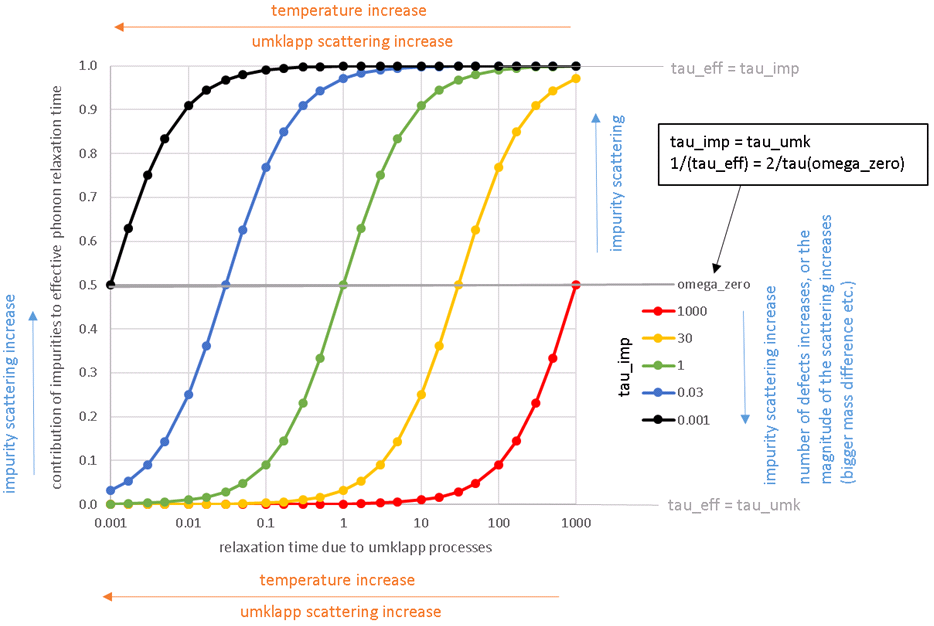
\includegraphics[width=\linewidth]{Figures/effective-phonon-relaxation-time.png}
  \caption{For a series of ${\tau}'$, their contribution to the effective phonon relaxation time is plotted against $\tau_{u}$. The quantity on the y-axis is the normalised difference in effective phonon relaxation time, comparing just Umklapp processes to Umklapp and the impurity scattering effect (as in Eq.~\ref{eq.Klemens7}). }
  \label{fig:relaxation_time}
\end{figure}

For a CMB-like condition of high temperature, Umklapp process relaxation time is short (left hand side of Fig. \ref{fig:relaxation_time}). Adding impurities (reducing ${\tau}'$) doesn't contribute much to an already large scattering effect. Where the Umklapp process relaxation time is longer (temperatures decreasing towards Debye temperature), even adding a small amount of atomic impurity can influence the effective system behaviour. Considering the average phonon velocity, a longer relaxation time means a greater distance travelled, or phonon mean free path.

Calling back to Equation \ref{eq.Klemens2} \& \ref{eq.Klemens3} , $A$ and $B$ are constants, where only the latter is temperature-dependent (T). The contribution of point defect scattering to the effective phonon relaxation time is constant with temperature (varying with impurity concentration and composition). It is the relative magnitude of $\tau_{u}$, which decreases with temperature ($\propto 1/T$, via $B$), to ${\tau}'$ that influences the effect of impurities on \tcs (see Equation \ref{eq.Klemens7}).
 
The two relaxation time terms above can be equated via Equation \ref{eq.Klemens11}, showing $\omega_{0}$ is similarily temperature-dependent
%
$$A{\omega_{0}}^{4}=B\left(T\right){\omega_{0}}^{2},$$
$${\omega_{0}}^{2}=B\left(T\right)/A\ ,$$
%
\begin{equation}
\omega_{0} \propto T\ .
\label{eq.Klemens23mod}
\end{equation}
%
The Debye frequency is a constant, so
%
\begin{equation}
\left (\frac{\omega_{\mathrm{0}}}{\omega_{\mathrm{D}}} \right ) \propto T\ .
\label{eq.Klemens23mod2}
\end{equation}
%
As temperature increases (above the Debye temperature), conductivity decreases because of Umklapp processes. The significance of point defect scattering (but not the magnitude of its relaxation time) decreases as the effect of phonon-phonon scattering increases. Therefore the relative conductivity decrease due to impurities is inversely proportional with temperature, and less important as conductivity tends towards its saturated minimum.



\pagebreak


%-----------------------------------------------------------
\section{Methodology}
%-----------------------------------------------------------

In this section I outline the process of taking Fe from chemistry to computer, by fitting my own coefficients to a Buckingham potential. I also go over how the Fe is incorporated into the \mgsio, considering its placement and concentration.

%---------------------------------------
\subsection{How does iron behave?} 
%---------------------------------------

I use two methods to introduce iron impurities to my bridgmanite models. The first approach is to simply create a magnesium atom with the mass of an iron atom, without changing any coefficients of the interatomic potentials from \citet{Oganov2000}. Despite being an obviously "quick and dirty" method, (I will show) this is a reasonable first-order approximation(((PROVE IT!?))). As the variation in mass number from Mg to Fe is large (24 to 56, a 133\% increase), it is likely to change the behaviour of the system more than a subtle change in the atomic interactions.

MENTION AMMANN IRON STUFF HERE

The second approach to add Fe into the \mgsios system is to fit interatomic potentials, as well as using the aforementioned mass change for a more realistic model. I adapted the \citet{Oganov2000} \mgsios Buckingham interatomic potential ($U$) to include the Fe-O interation. I determined two short-range potential parameters, $b$ and $\rho$, shown in Eq. 11 from \citet{Oganov2000},
%
\begin{equation}
U_{ij}\left ( R_{ij} \right ) = \frac{z_{i}z_{j}}{R_{ij}} + b_{ij}\ \textup{exp}\left ( - \frac{R_{ij}}{\rho_{ij}} \right ) - \frac{c_{ij}}{{R_{ij}}^{6}}, \label{og_buck}
\end{equation}
%
where $ij$ refers to an atom pair, $R$ is interatomic distance, $z$ is atomic charge, and $c$ relates to the Van der Waals force (zero for non O-O interactions). We determine $\rho$ in the same fashion as \citet{Oganov2000}, calculated from the atomic first ionisation potentials,
%
\begin{equation}
\rho_{ij} = \frac{1.85}{\sqrt{I_{i}}+\sqrt{I_{j}}}.  \label{urusov}
\end{equation}
%
$b$ is constrained using the GULP code \citep{Gale1997}, using the calculated $\rho$ value for Fe-O. We fit to the elasticity results of \citet{Parise1990}, an experimental study of (Mg$_{0.9}$,Fe$_{0.1}$)SiO$_3$ bridgmanite up to 433~K. Despite potential fitting being an improvement on solely changing mass (((PROVE IT!?))), it is still not perfect as the charge of our fitted Fe is not varied from the original Mg.

!!! Validate potentials

!!! Validate Fe vs. heavy Mg, isotope mass

!!! Include Oganov table (earlier?), with the fitted Fe info


%---------------------------------------
\subsection{Where do the impurities go?} 
%---------------------------------------

Iron is substituted with magnesium into the bridgmanite atomic structure. The unit cell contains 4~Mg atoms, and the smallest direct method cell I employ is a 6x2x2 supercell. Therefore the smallest amount of iron that can be added is 1/96 atoms, a concentration just over 1\%. A simple MATLAB script (((REF, APPENDIX))) is used to modify LAMMPS input files, randomly selecting a specified proportion of Mg atoms to be replaced with Fe. When a Mg atom changes to Fe, its mass and interatomic potential properties change. 

Due to the microscopic nature of the system, we do not want all of the added iron to be concentrated together in the simulation cell, especially in a heat source/sink region (((ELABORATE WITH FIGURE?))). To avoid this we order Mg atoms by length along supercell, and change a single atom every so many. For example, changing 1/4 atoms is different to changing 24/96. The latter has a higher variance in Fe per unit length, and the former chooses one atom to swap for every four along the system. After iron is added, the standard direct method or Green-Kubo workflow is followed.

!!! NICE PICTURE/DIAGRAM HERE?

!!! Comparison of random and homogeneous distribution, don't make reader engage their imagination, show obvious picture




%-----------------------------------------------------------
\section{Results}
%-----------------------------------------------------------

% reference SS2015 supp. for this section, the what affects conductivity bit
% have I gone too far into discussion here, interpretation of results?
Lattice thermal conductivities obtained from Green-Kubo calculations are plotted against temperature in Figure \ref{fig:kappa-temp_01}, for Mg and Fe-endmembers and the 50/50 solid solution mix.

Conductivity decreases with temperature, approximately following $\kappa \propto 1/T^{0.9}$ at the pressure of 136~GPa considered here. This is in contrast to the typically expected $\kappa \propto 1/T$ relation, indicating some kind of saturation in conductivity decrease with temperature.

\fesios has a consistently lower conductivity than \mgsio, although both species may converge given a high enough, albeit unphysical, lower mantle temperature. This suggests there is a minimum conductivity associated with the crystal structure, reached first by \fesios with its inherently lower conductivity.

The 50\% solid solution has a consistently lower conductivity than \mgsio, and a lower than or equal to relation to \fesios. This is again to be expected, conductivity decreases from endmember to intermediate compositions as inpurity concentration increases. It can be seen that conductivity differences are very small at high temperatures for \fesios and the solid solution. If \fesios has already reached its theoretical minimum, adding impurities will do little to decrease it further.

\begin{figure}[h!]
  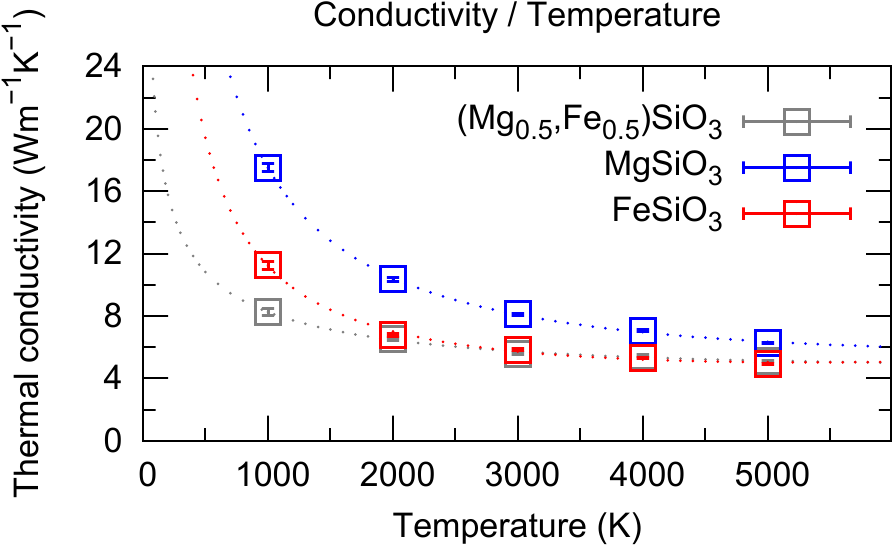
\includegraphics[width=\linewidth]{Figures/k-t_all_02.png}
  \caption{Data points are GK conductivity results, dotted line is the fit from Equation \ref{eq.okuda5modmod}.}
  \label{fig:kappa-temp_01}
\end{figure}

An alternative perspective to Figure \ref{fig:kappa-temp_01} is presented in Figure \ref{fig:kappa-comp_01}, where Green-Kubo conductivity results are plotted as a function of Fe impurity content for several temperature series.

Conductivity generally decreases with increasing temperature at all compositions, though the change becomes minimal at tempertatures above 3000~K.

The \mgsios endmember has a consistently higher conductivity than the \fesio. This can be explained by the general reduction in shear modulus and increase in density associated with adding Fe, which decreases seismic velocity and thus conductivity [[[TRUTH ALERT, REF???]]].

The amount of Mg atoms replaced with Fe has a variable effect on conductivity. A better way to label the effect is impurities added to an endmember, i.e. Fe is added to \mgsios and Mg to \fesio, which always serves increase phonon scattering and decrease conductivity. The decrease from this effect saturates towards a 50\% compositional mix. At high temperatures, this effect is minimal when adding Mg to \fesio. The conductivity could already be close to its theoretical minimum due to temperature effects, little reduction is observed from adding impurities.

\begin{figure}[h!]
  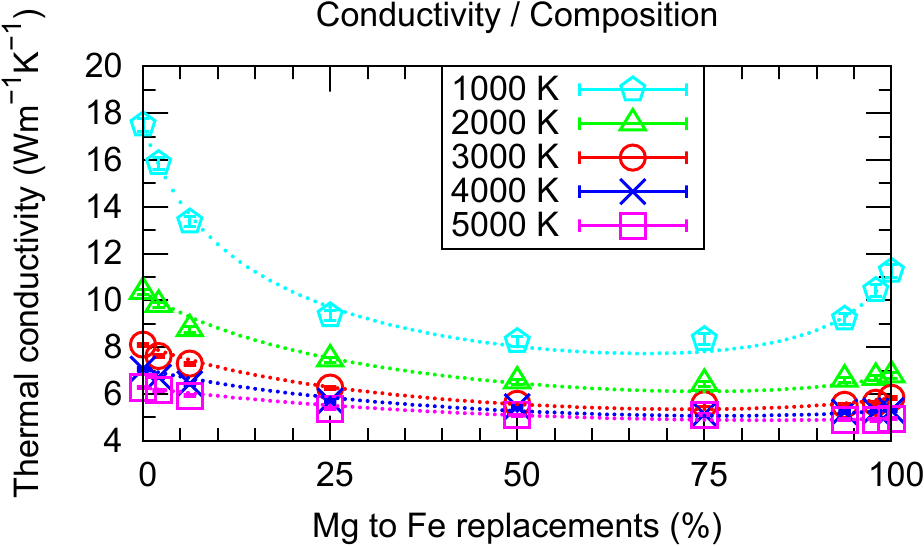
\includegraphics[width=\linewidth]{Figures/k-c_all_01.png}
  \caption{CAPTION}
  \label{fig:kappa-comp_01}
\end{figure}

A simple interpolation between endmember conductivities is insufficient, the presence of a compositional mix has an effect. This effect is itself temperature-dependent, the trough-like trend flattens with increasing temperature. These temperature and compositional dependences can be combined, allowing conductivity to be determined for a range of possible CMB conditions (Figure \ref{fig:kappa-temp-comp_01}). 

\begin{figure}[h!]
  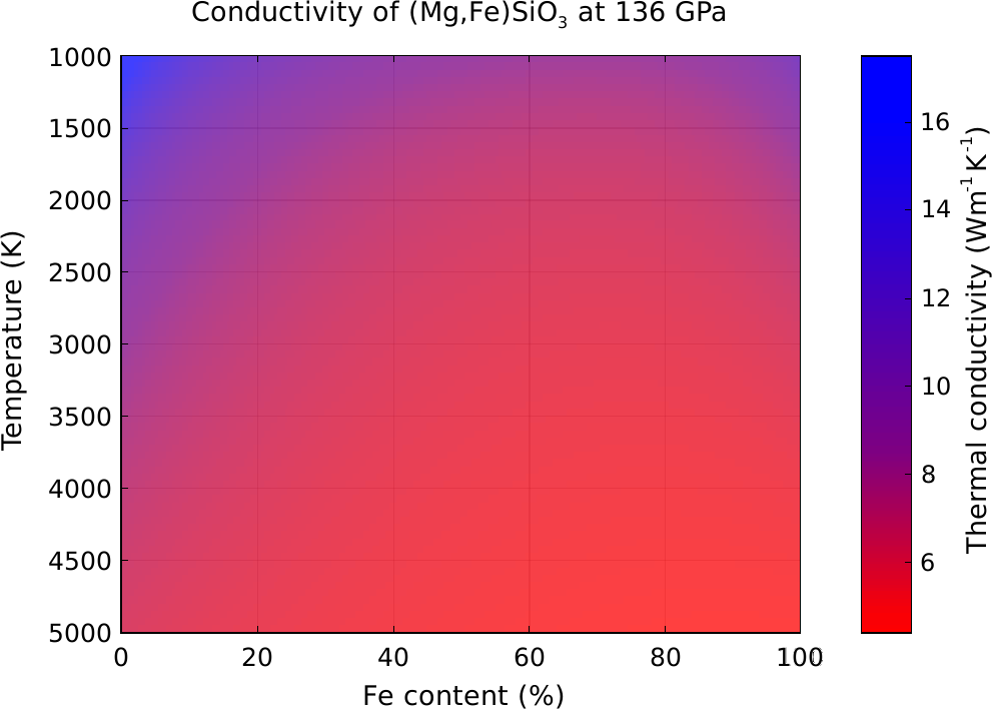
\includegraphics[width=\linewidth]{Figures/K_over_T_over_X.png}
  \caption{Modelled conductivity, shown plotted against temperature and composition. Note the sensitivity of the colour scale, showing low conductivities as dominant at high temperatures and intermediate compositions. High values are found only at low temperatures, and even then they rapidly decay and saturate to <8\wmk. Such conditions are unphysical at 136~GPa within the lower mantle.}
  \label{fig:kappa-temp-comp_01}
\end{figure}



%-----------------------------------------------------------
\section{Parameterising the effect of composition and temperature on CMB conductivity}
%\section{Making the mantle model}
%-----------------------------------------------------------

In this section I develop a model for the lattice thermal conductivity of \mgfesios perovskite at CMB conditions. Whilst the CMB is a small section of the lower mantle, it marks the heat flow boundary from core to mantle. Mantle-side thermal conductivity controls the nature of this heat flow, making it an important parameter in studies on both sides of a an important interface. The CMB is isobaric at 136~GPa, and isothermal at an uncertain temperature. Fe-content can vary with position. In terms of making a model I can collect data at one pressure condition, and investigate how an array of temperatures and compositions affect \tc.

Due to uncertainty in the lower mantle's composition, properties like \tcs are often averaged considering the abundance of each mineral component. There are also solid solutions to consider though, particularly the concentration of Fe in \mgsio, as well as the phase boundary between bridgmanite and \mgsios post-perovskite. 

The conductivity of an intermediate composition is not a simple weighted average of the endmember values, you cannot interpolate linearly. This can be seen in Figure \ref{fig:kappa-temp_01}, where the (Mg$_{0.5}$,Fe$_{0.5}$)SiO$_3$ results do not plot between those of \mgsios and \fesio.



%%%%%%%%%%%%%%%%%%%%%%%%%%%%%%

%---------------------------------------
\subsection{Parameterising the data fit} 
%---------------------------------------

[Equations from \cite{Ohta2017} (eq. 7,8,9), and \cite{Okuda2017} (eq. 5)]

Equations and functional forms exist for the temperature and compostional dependence of \tc, and it is possible to combine the two. The basic idea is to determine the conductivity of \mgsios and \fesios endmembers at the temperature of interest, and then apply the (temperature-dependent) effect of composition.

\citet{Padture1997} propose a model for how impurities affect lattice thermal conductivity of a solid soultion, which \citet{Ohta2017} use to fit experimental ferropericlase data. Following a similar methodology, I fit the functional form to my (Mg,Fe)SiO$_3$ perovskite results at various temperatures (1000~K, 2000~K, 3000~K, 4000~K, and 5000~K). In an additional step, I establish how the functional forms change with temperature, the temperature-dependence of the compositional-dependence if you will.

\citet{Okuda2017} present a temperature scaling relation for lattice conductivity \citep[originally from][]{Manthilake2011}, fit to their experimental results of bridgmanite. I apply this temperature scaling to computational results of \mgsios and \fesios at 136~GPa. With the temperature dependence of these endmembers and of the compositional effect, I am able to able to determine the conductivity of any composition, interpolating to temperatures in the range 1000~K to 5000~K, at 136~GPa pressure representative of the CMB.

The aforementioned temperature dependence from \citet{Manthilake2011} considers density, allowing conductivity to be determined as a function of temperature and pressure. In the examples I will present, I am only concerned with systems at 136~GPa. All density changes will result from thermal expansion, and the equations will be altered to accomodate this.

Some of the equations in the following section have already been presented as analogous forms in Section \ref{impur_theory}. The equations are kept similar to their published form, which was \citet{Stackhouse2015} in the former, and \citet{Ohta2017, Okuda2017} in the following.

%\pagebreak
%    
%%-------------------
%\subsubsection{Compositional dependence}
%%-------------------
%
%\citet{Ohta2017} Eq.~7
%\begin{equation}%-----
%\kappa_{latt}=\kappa_{i}\left ( \frac{\omega_{0}}{\omega_{M}} \right )\mathrm{arctan}\left ( \frac{\omega_{M}}{\omega_{0}} \right )
%\label{eq.ohta7}
%\end{equation}%-------
%\\ $\kappa_{latt}$ - output conductivity as function of t \& x (\wmk), considering mineral specific parameters\\
%$\kappa_{i}$ - the composition-dependent conducitivity, if it were linearly interpolated between endmembers (\wmk)\\
%$\omega_{0}$ - \enquote{\textit{the phonon frequency where the intrinsic mean free path is equal to that due to solute atoms (or just interatomic spacing?)}}\\
%$\omega_{M}$ - \enquote{\textit{the phonon frequency corresponding to the maximum of the acoustic branch of the phonon spectrum (Debye frequency)}}\\
%
%The two components $\kappa_{i}$ and $\omega_{0}/\omega_{M}$, are both temperature and composition-dependent. $\kappa_{i}$ gives the compositionally-weighted average conductivity, a linear interpolation between endmembers at a certain temperature. $\omega_{0}/\omega_{M}$ controls the conductivity decrease due to the impurity effect, the magnitude of which depends on the temperature and composition of interest.
%
%By combining models for the temperate-dependence of \mgsios and \fesio-endmember conductivities, and the fit $\chi^{T}$ parameter, I obtain a function for conductivity of the lower mantle (136~GPa) as a function of just temperature and composition (as illustrated in Figure. \ref{fig:kappa-comp_01}).\\
%
%
%
%
%Ohta eq. 8 
%\begin{equation}%-----
%\left ( \frac{\omega_{0}}{\omega_{M}} \right )^{2}=\frac{\chi^{T}}{C\left ( 1-C \right )}  
%\label{eq.ohta8}
%\end{equation}%-------
%$\omega_{0}$ - \enquote{\textit{the phonon frequency where the intrinsic mean free path is equal to that due to solute atoms (or just interatomic spacing?)}}\\
%$\omega_{M}$ - \enquote{\textit{the phonon frequency corresponding to the maximum of the acoustic branch of the phonon spectrum (Debye frequency)}}\\
%$\chi^{T}$ -temperature-dependent parameter to \dots ??? \\
%$\chi$ - \enquote{\textit{a constant}}\dots\\
%$T$ - temperature of interest (K, default data fit between 1000 - 5000 K, but extrapolation should be reasonable)\\                    
%$C$ - composition mix of interest (dimensionless, values between 0 and 1)\\
%
%The equation splits $\omega_{0}/\omega_{M}$ into its temperature and composition-dependent components, where $\chi$ is a temperature-dependent variable. A value for $\chi$ is fit for all compositions at each temperature. $C\left ( 1-C \right )$ is largest when $C=0.5\ or\ 50\%$, relating to the shape of the trough formed by this fit.\\
%
%$\chi^{T}$ scaling 
%\begin{equation}%-----
%\chi^{T}=A T^{B}
%\label{eq.chi_scale}
%\end{equation}%-------
%\\ *$\chi^{T}$ -temperature-dependent parameter to \dots ??? \\
%*$\chi$ - \enquote{\textit{a constant}}\dots\\
%*$T$ - temperature of interest (K, default data fit between 1000 - 5000 K, but extrapolation should be reasonable)\\                    
%$A$ - coefficient in $\chi^{T}$ variation with temperature\\
%$B$ - exponent in $\chi^{T}$ variation with temperature\\
%
%In order to obtain an equation for conductivity at any mantle temperature, it is required that $\chi$ can be expressed as function of temperature. Figure \ref{fig:draft_xt} shows $\chi$ over $T$ fit with a power law and 4th order polynomial, the former of which is a poor fit and the latter an egregious overfitting. 
%
%\begin{figure}[h]
%  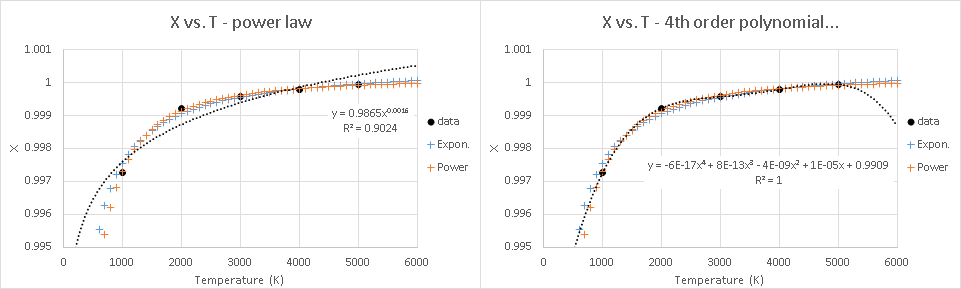
\includegraphics[width=\linewidth]{Figures/draft_XT.png}
%  \caption{The fit $\chi$ values plotted against $T$, with power law (left) and 4th order polynomial (right) trendlines. Blue and orange series are the exponential and power law fits obtained from plotting $\chi^T/T$ (see Figure \ref{fig:draft_xtt}).}
%  \label{fig:draft_xt}
%\end{figure}
%
%The lack of an obvious trend in $\chi$ against $T$ can be countered by plotting $\chi^T$ over $T$, and fitting either a expontial or power law relationship (Figure \ref{fig:draft_xtt}). I use the power law-relationship as it represents the temperature-dependence better, both statistically and sensitivity-wise. The value of $\chi^T$ at high $T$ has a lesser effect on the conductivity-composition relationship than at low $T$, where the power law fit matches the data closer. In Figure \ref{fig:draft_xt}, we can see that either of the power law or exponential $\chi^T/T$ fits represent the data better than the $\chi/T$ relations.\\ 
%
%\begin{figure}[h]
%  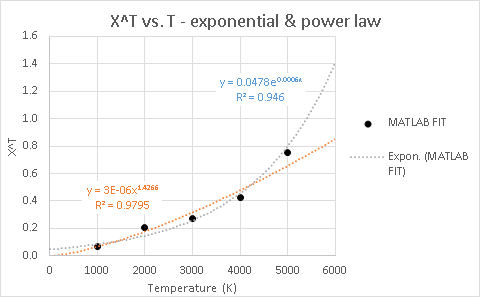
\includegraphics[width=\linewidth]{Figures/draft_XTT.png}
%  \caption{Exponential fit in blue (more curved), power law in orange (flatter)}
%  \label{fig:draft_xtt}
%\end{figure}
%
%
%
%Ohta eq. 9 
%\begin{equation}%-----
%\kappa_{i}=\left ( 1-C \right )\kappa_{\mathrm{MgSiO_{3}}}+C\ \kappa_{\mathrm{FeSiO_{3}}}
%\label{eq.ohta9}
%\end{equation}%-------         
%\\ *$\kappa_{i}$ - the composition-dependent conducitivity, if it were linearly interpolated between endmembers (\wmk)\\
%*$C$ - composition mix of interest (dimensionless, values between 0 and 1)\\
%$\kappa_{MgSiO_{3}}$ - temperature and volume-dependent conductivity for Mg endmember (\wmk)\\
%$\kappa_{FeSiO_{3}}$ - temperature and volume-dependent conductivity for Fe endmember (\wmk)\\
%
%This equation describes the conductivity of an intermediate composition, assuming the relation is a simple weighted mean. $C$, in this case specifically, is the proportion of Fe atoms swapped into the system for Mg. The actual dependence of conductivity with composition is more complicated, this intermediate average value is adjusted for atomic-scale effects in Equation.~\ref{eq.ohta7} \citep[][Eq. 7]{Ohta2017}. \\
%
%%-------------------
%\subsubsection{Temperature dependence}
%%-------------------
%
%\cite{Okuda2017}\\
%
%Okuda eq. 5 
%
%\begin{equation}%-----
%\kappa_{adj}=\kappa_{\mathrm{ref}}\left ( \frac{\rho}{\rho_{\mathrm{ref}}} \right )^{g}\left ( \frac{T_{\mathrm{ref}}}{T} \right )^{a}
%\label{eq.okuda5}
%\end{equation}%-------
%\\ $\kappa_{adj}$ - temperature and density-dependent conductivity of an endmember (\wmk)\\
%$\kappa_{ref}$ - reference conducitivty\\
%$T_{ref}$ - reference temperature\\
%$a$ - exponent controlling temperature-dependent conducitvity of an endmember\\
%$\rho_{ref}$ - reference density\\
%$g$ - exponent controlling density-dependent conducitvity of an endmember\\
%
%\citet{Okuda2017} use a model for density and temperature-dependent conductivity (((from Manthilake 2011, REF???))), which utilises exponents obtained from REAL data / is calculated? (actually real numbers, only mine are fitted?). A reference value is scaled to infer conductivity at the conditions of interest, which in this case is temperature and pressure (via proxy using simulation cell volume/density).\\
%
%
%
%Okuda eq. 5 modified
%
%\begin{equation}%-----
%\kappa_{\mathrm{adj}}=\kappa_{\mathrm{ref}}\left ( \frac{T_{\mathrm{ref}}}{T} \right )^{a}\left ( \frac{V_{\mathrm{ref}}}{V} \right )^{g}
%\label{eq.okuda5_mod}
%\end{equation}%-------
%\\ $T_{\mathrm{ref}}$ - temperature at which reference conductivity is calculated (K)\\
%$T$ - temperature of interest to interpolate (K, default data fit between 1000 - 5000 K, but extrapolation should be reasonable)\\   
%$V_{\mathrm{ref}}$ - reference volume of an endmember (E-30 m$^3$)\\
%$V$ - temperature-dependent volume of an endmember (E-30 m$^3$)\\
%$h$ - exponent controlling volume-dependent conducitvity of an endmember\\
%
%I adapt Eq. \ref{eq.okuda5} to consider volume instead of density (Eq. \ref{eq.okuda5_mod}), where density and volume are inversely proportional. Varying $a$ and $h$ I fit this equation for both Mg and Fe endmembers, using reference values from 1000~K (see Figure \ref{fig:kappa_temp_01}). The purpose of this is to scale the conductivities needed for Eq. \ref{eq.ohta9} to any temperature of interest.
%
%\pagebreak
 
%-------------------
\subsubsection{Compositional dependence}
%-------------------

REFERENCE BACK TO METHODOLOGY FOR FIRST TWO EQUATIONS AND DEFINITIONS ETC.

The lattice thermal conductivity of a solid-solution as a function of temperature and composition can be approximated by the following equation,
%
WHY DOES THIS EQUATION EVEN WORK?
%
\begin{equation}
\kappa_{\mathrm{SS}}=\kappa_{\mathrm{V}}\left ( \frac{\omega_{\mathrm{0}}}{\omega_{\mathrm{D}}} \right )\mathrm{arctan}\left ( \frac{\omega_{\mathrm{D}}}{\omega_{\mathrm{0}}} \right ),
\label{eq.ohta7}
\end{equation}
%
where $\omega_{\mathrm{0}}$ is the phonon frequency at which the Umklapp/regular processes and impurity scattering effects' contributions to the mean free path and relaxation time (distance and time respectively travelled by a phonon) are equal. In terms of generating thermal resistance, neither effect dominates over the other at this frequency. $\omega_{\mathrm{D}}$ is the phonon frequency corresponding to the maximum of the acoustic branch in the phonon spectrum (the Debye frequency). $\kappa_{\mathrm{V}}$ is the conductivity of the solid solution in the absence of impurity scattering
%
\begin{equation}
\kappa_{\mathrm{V}}=\left ( 1-C \right )\kappa_{\mathrm{MgSiO_{3}}}+C\ \kappa_{\mathrm{FeSiO_{3}}}\ ,
\label{eq.ohta9}
\end{equation}
%
where $C$ is the fractional concentration of Fe, and $\kappa_{\mathrm{MgSiO_{3}}}$ and $\kappa_{\mathrm{FeSiO_{3}}}$ the temperature dependent conductivities of the endmembers. The ratio of the phonon frequencies can be expressed as

WHAT IS THE THEORY BEHIND THIS?
%
\begin{equation}
\left ( \frac{\omega_{\mathrm{0}}}{\omega_{\mathrm{D}}} \right )^{2}=\frac{\chi^{T}}{C\left ( 1-C \right )}\ ,
\label{eq.ohta8}
\end{equation}
%
where $\chi$ is a temperature-dependent constant, and $T$ is the temperature of interest. $\chi$ can be thought of as a measure of resistance to the effects of impurity scattering. The $\kappa$ against $C$ relationship (Figure~\ref{fig:kappa-comp_01}) shows a larger effect of impurity scattering in the form of greater curvature when $T$ and $\chi$ are lower (see Table \ref{tab:temp-table}). For a given $T$ and $C$, increasing $\chi$ causes the phonon frequency ratio $\left ( \frac{\omega_{\mathrm{0}}}{\omega_{\mathrm{M}}}\right )$ to increase which, as discussed in Section \ref{impur_theory}, means $\kappa_{\mathrm{latt}}$ tends towards $\kappa_{\mathrm{i}}$. $\chi$ is fit to the data at each temperature, but for the model we need it as a function of temperature. Figure \ref{fig:draft_xt} shows a plot of $\chi$ against $T$ with a power law (LEFT/B.) and 4th-order polynomial (RIGHT/B.), the former of which is a poor fit and the latter an egregious overfitting. 

%-----------------------------------------------------------
\begin{table}[h!]
\begin{tabular}{cc|lllll}
                                                                           &       & \multicolumn{5}{c}{Temperature (K)}                       \\

                                                                           &       &  1000  & 2000    & 3000    & 4000    & 5000 \\ \hline

\multirow{2}{5em}{Conductivity (\wmk)}     & Mg & 17.51  & 10.36   & 8.11     & 7.07     & 6.28 \\ 

                                                                           & Fe   & 11.26  & 6.79     & 5.84     & 5.30     & 4.95 \\ \hline

\multirow{2}{*}{Volume (\AA$^{3}$)}          & Mg & 5960   & 6017    & 6075    & 6136    & 6199 \\

                                                                           & Fe   & 6253   & 6310    & 6369    & 6431    & 6500 \\ \hline
                                                                           
\multirow{2}{*}{$V_{\mathrm{ref}}/V(T)$}  & Mg & 1         & 0.9906 & 0.9811 & 0.9714 & 0.9616 \\
                                                                           
                                                                           & Fe   & 1         & 0.9909 & 0.9817 & 0.9723 & 0.9619 \\ \hline
                                                                           
\multicolumn{2}{c|}{$\chi$}                                     & 0.9973 & 0.9992 & 0.9996 & 0.9998 & 0.9999 \\

\multicolumn{2}{c|}{$\chi^{T}$}                            & 0.0649 & 0.2035 & 0.2748 & 0.4277 & 0.7494
\end{tabular}
\caption[]{\label{tab:temp-table}}
\end{table}
%-----------------------------------------------------------

\begin{figure}[h!]
  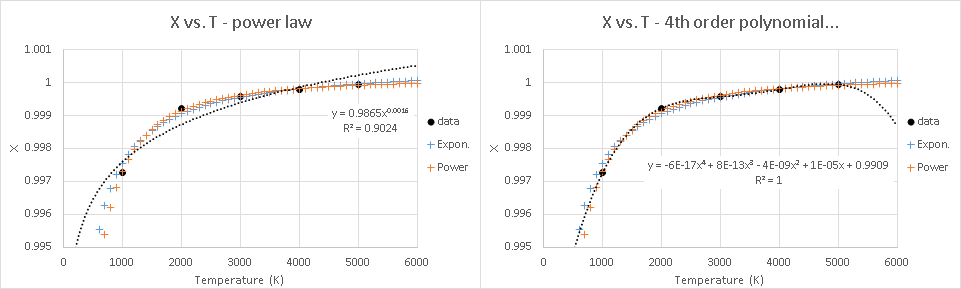
\includegraphics[width=\linewidth]{Figures/draft_XT.png}
  \caption{The fit $\chi$ values plotted against $T$, with power law (LEFT/A.) and 4th order polynomial (RIGHT/B.) trendlines (both black). Blue and orange series are the exponential and power law fits obtained from plotting $\chi^T/T$ (see Figure \ref{fig:draft_xtt}).}
  \label{fig:draft_xt}
\end{figure}

The lack of an obvious trend in $\chi$ against $T$ can be mitigated by plotting $\chi^T$ over $T$, and fitting either a expontial or power law relationship (Figure~\ref{fig:draft_xtt}). I use the following power law-relationship, 
%
\begin{equation}%-----
\chi^{T}=A T^{B},
\label{eq.chi_scale}
\end{equation}%-------
%
where $A$ is the coefficient and $B$ is the exponent to be determined. The magnitudes of these fit parameters are $3.468 \times 10^{-6}$ and $1.426$ respectively. This fit represents the temperature-dependence better, both statistically and sensitivity-wise compared to an exponential relationship $\left ( \chi^{T}=A e^{BT}\right )$. The value of $\chi^T$ at high $T$ has a lesser effect on the conductivity-composition relationship than at low $T$, where the power law fit matches the data closer. In Figure~\ref{fig:draft_xt}, we can see that both the power law and exponential $\chi^T$ over $T$ relationships fit the data better than the $\chi$ over $T$ power law or polynomial relations.

\begin{figure}[h]
  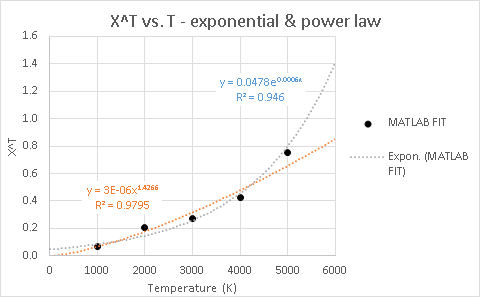
\includegraphics[width=\linewidth]{Figures/draft_XTT.png}
  \caption{Exponential fit in blue (more curved), power law in orange (flatter)}
  \label{fig:draft_xtt}
\end{figure}

The conductivities of $\kappa_{\mathrm{MgSiO_{3}}}$ and $\kappa_{\mathrm{FeSiO_{3}}}$ from Equation \ref{eq.ohta9} can be scaled with temperature, giving an adjusted value 
%
\begin{equation}
\kappa_{\mathrm{adj}}=\kappa_{\mathrm{ref}}\left ( \frac{\rho}{\rho_{\mathrm{ref}}} \right )^{g}\left ( \frac{T_{\mathrm{ref}}}{T} \right )^{a}.
\label{eq.okuda5}
\end{equation}
%
$\rho$ is density, $g$ and $a$ are exponents which control the nature of the density and temperature-dependence, and ``ref'' denotes a reference value. This equation is fit to the data, anchored around the values of the reference data point (the fit is shown in Figure~\ref{fig:kappa-temp_01}). I fit to the data point at 1000~K, as the conductivities at higher temperatures become more similar, converging towards a minimum point. Anchoring to 1000~K reduces the error in the fit, on account of the relatively larger conductivity at this temperature. BIGGER VALUE, IS THE ERROR RELATIVE TO THE VALUE SMALLER?

For a given composition, the mass of the simulated system does not change with temperature. The number and type of atoms remains constant, while thermal effects cause density variations. The density relation in Equation~\ref{eq.okuda5} can be reformulated as
%
\begin{equation}
\frac{\rho }{\rho _{\mathrm{ref}}} \equiv \frac{V_{\mathrm{ref}}}{V} \ ,
\label{eq.rho_to_vol}
\end{equation}
%
because $\rho \propto V^{-1}$, where $V$ is the volume of the system in question. This leads to a modified version of Equation~\ref{eq.okuda5}
%
\begin{equation}
\kappa_{\mathrm{adj}}=\kappa_{\mathrm{ref}}\left ( \frac{V_{\mathrm{ref}}}{V} \right )^{g}\left ( \frac{T_{\mathrm{ref}}}{T} \right )^{a}.
\label{eq.okuda5mod}
\end{equation}

The exponent $g$ represents the rate of change of lattice thermal conductivity with density, at a constant temperature,
%
\begin{equation}
g=\left( \partial \ln \kappa_{\mathrm{latt}} / \partial \ln \rho \right) _{T} \ .
\label{eq.g_def}
\end{equation}
%
The density/volume changes that I observe result from thermal effects, i.e. not at a constant temperature and not pressure-driven. The rate of change in conductivity with density in my data are better represented as something like 
%
\begin{equation}
h \sim \left( \partial \ln \kappa_{\mathrm{latt}} / \partial \ln \rho \right) _{P} \ ,
\label{eq.g_def}
\end{equation}
%
where pressure ($P$) is the condition kept constant. The significance here is that pressure-driven and temperature-driven density changes affect the conductivity differently. At constant temperature, conductivity and density increase with pressure. The opposite is true at constant pressure for the material and temperatures considered here, conductivity and density decrease with increasing temperature. The result is $g$ and $h$ having opposite polarities based on the scenarios they describe.

Volume does not need to be input ((INDEPENDENT?)) variable for the model, as all the data are obtained from constant pressure (136~GPa) calculations and any volume variations relate to thermal expansion. I express the volume ratio shown in Equation~\ref{eq.okuda5mod} as 
%
\begin{equation}
\frac{V_{\mathrm{ref}}}{V(T)} \approx  mT+c \ ,
\label{eq.linear_v_mT_c}
\end{equation}
%
a simple linear function of temperature (see Figure~\ref{fig:draft_VrefV-T}), where $m$ is the gradient and $c$ the intercept (as you might expect). 

\begin{figure}[h!]
  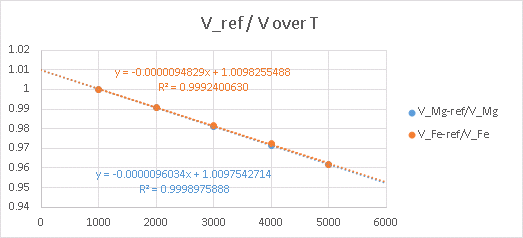
\includegraphics[width=\linewidth]{Figures/draft_VrefV-T.png}
  \caption{$V_{\mathrm{ref}}/V$ can be expressed as a simple linear function of $T$.}
  \label{fig:draft_VrefV-T}
\end{figure}

With Equation~\ref{eq.linear_v_mT_c}, we rewrite Equation~\ref{eq.okuda5} one more time,
%
\begin{equation}
\kappa_{\mathrm{adj}}=\kappa_{\mathrm{ref}} \left ( mT+c \right )^{h} \left ( \frac{T_{\mathrm{ref}}}{T} \right )^{a}.
\label{eq.okuda5modmod}
\end{equation}
%
This equation allows me to obtain a conductivity value at any temperature within the fit range, comprising a reference conductivity and temperature for the material in question, with constants ($m$, $c$, $h$, \& $a$, see Table \ref{tab:comp-table}) fit to data across a range of temperatures. This scaling process is necessary for $\kappa_{\mathrm{MgSiO_{3}}}$ and $\kappa_{\mathrm{FeSiO_{3}}}$, which have their own reference values and fit constants.

%-----------------------------------------------------------
\begin{table}[]
\begin{tabular}{c|ccc}
                           & \multicolumn{3}{c}{Composition}    \\
                           & Mg             & SS           & Fe           \\ \hline
$\kappa_{ref}$  & 17.51         & 8.26        & 11.26      \\
$h$                     & -10.93        & -5.52       & -17.32     \\
$a$                     & 0.896         & 0.428       & 0.913     \\
$m$                    & -9.60E-06  & -9.47E-06 & -9.48E-06 \\
$c$                      & 1.00975    & 1.00965    & 1.00983
\end{tabular}
\caption[CONTENTS BIT?]{\label{tab:comp-table}Mg and Fe refer to \mgsios and \fesios endmembers, SS the solid solution with a 50\% mix.}
\end{table}
%-----------------------------------------------------------






ADD MORE REFEERENCES DUH








%Volume scaling ($y=mx+c$)  

%\begin{equation}%-----
%V=\frac{\partial V}{\partial T} T+V_{T_{0}}
%\label{eq.vol_scale}
%\end{equation}%-------     
%\\ *$V$ - temperature-dependent volume of an endmember (E-30 m$^3$)\\          
%${\partial V}/{\partial T}$ - fit gradient, change of volume with temperature (E-30 m$^3$/K)\\
%*$T$ - temperature of interest (K, default data fit between 1000 - 5000 K, but extrapolation should be reasonable)\\
%$V_{T_{0}}$ - intercept volume for T=0~K (E-30 m$^3$)\\

%I take Eq.~\ref{eq.okuda5} \citep[][Eq. 5]{Okuda2017} a step further, by obtaining $V$ in terms of $T$. This dependence is effectively linear over the temperatures considered (see Figure \ref{fig:draft_vt}). With this, Eq. \ref{eq.okuda_mod} can be made into a function of just temperature, meaning Eq.~\ref{eq.ohta7} \citep[][Eq. 7]{Ohta2017} is dependent solely on temperature, composition, and fit or calculated constants.

%\begin{figure}[h]
%  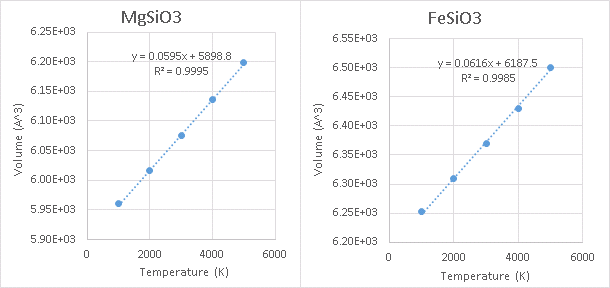
\includegraphics[width=\linewidth]{Figures/draft_VT.png}
%  \caption{Number of atoms is kept constant for all volumes, data is obtained from GK calculations of a 4x4x3 simulation cell. Magnitude of volume isn't of interest, just the relative difference to the reference volume.}
%  \label{fig:draft_vt}
%\end{figure}



\pagebreak


